\section{An illustrative example}
\label{Buildingblocks}
We illustrate the tradeoffs involved in implementing a packet-processing
pipeline on general-purpose
hardware, using an example of the L2 packet forwarding application.
At the high-level specification, the application involves input streams
of packets (one stream per input NIC) converging
to a processing node that looks up the packets' MAC addresses (source
and destination)
to index locally-stored lookup tables, to decide the destination of the packet, and
output streams of packets (one stream per output NIC) emerging out of
the processing node. We use
this simple application to illustrate the performance implications of
scheduling and prefetching decisions made by the compiler. We focus on performance
optimization for a single CPU core. Multi-queueing support in modern NICs
ensures that most applications can scale near-linearly with the number of cores.
\begin{figure}[ht]
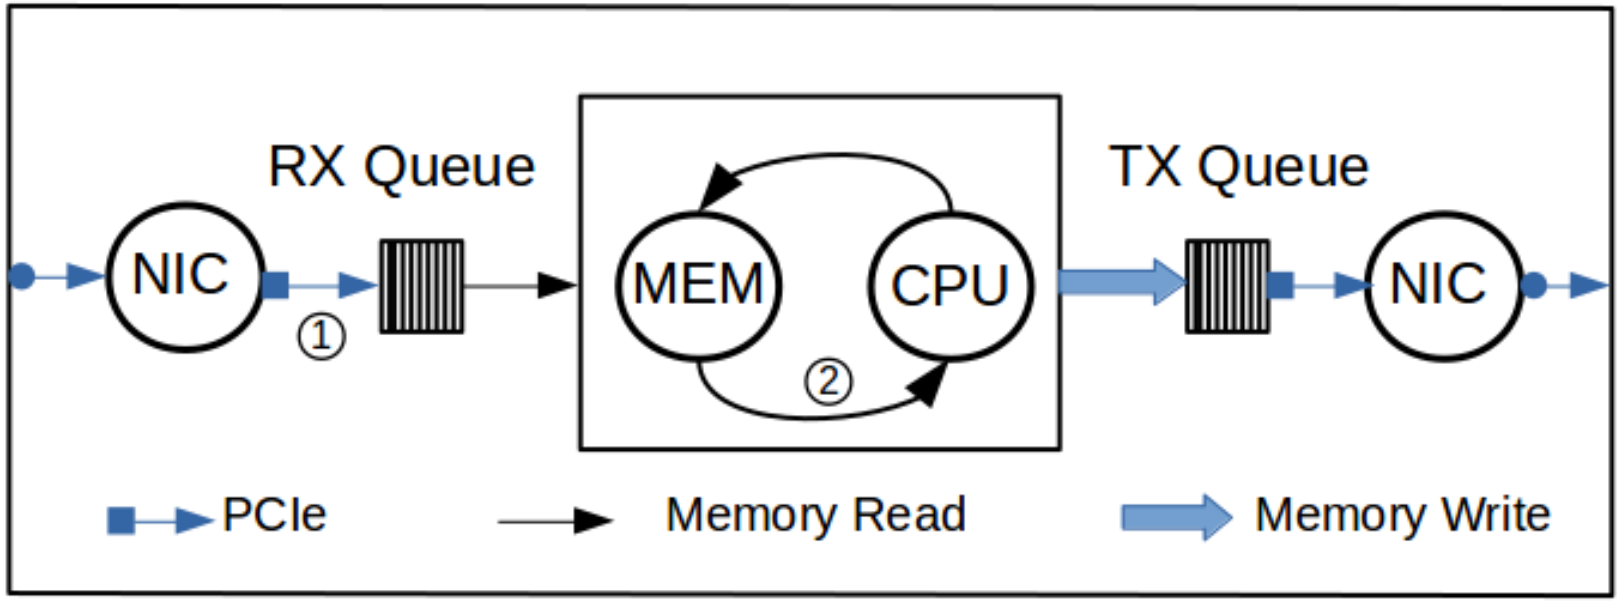
\includegraphics[width = \linewidth]{Figures/queuing.png}
\caption{Packet Processing Pipeline}
\label{fig:overviewfigure}
\end{figure}


We first discuss the characteristics of the underlying hardware.
Three components of a general-purpose architecture, are most critical to the performance of the
packet-processing
application: NIC subsystem, CPU, and Memory subsystem. Figure~\ref{fig:overviewfigure}
illustrates the data-flow at the hardware level. The NIC is involved in reading the packets
off the wire and storing them into main memory. In our experiments, a NIC's input bandwidth
is upper-bounded by 10Gbps, however, its bandwidth to memory is usually much higher\footnote{The
total PCIe bandwidth to main memory in our experiments
is around 8 GT/s, which gets shared across multiple NICs. For
all our experiments, except one (IPv4), the total PCIe bandwidth remains unsaturated.}. The latency
from NIC to main memory is usually long (i.e., the NIC-memory DMA interface is a high-bandwidth
high-latency interface), and so it is important to allow multiple
packets in flight from NIC to memory, to ensure effective bandwidth utilization across the
NIC-memory DMA interface. To realize this parallelism, we need {\em batching}, by ensuring
that multiple
packets are consumed/produced to the NIC's ring buffer in one shot. This allows the NIC to initiate
multiple PCIe transactions in parallel, thus hiding the round-trip NIC-memory latency. This
available parallelism at the NIC-memory interface is labeled as \textcircled{1}
in Figure~\ref{fig:overviewfigure}.

The next step in each packet processing pipeline is the actual logic.
Some applications are CPU-bound (involve
significant processing time), and others are memory-bound (involve significant cache-misses
and round trips to main memory). If an application is CPU bound, we cannot do much, and rely
on the underlying C compiler to tighten the code, and extract the SIMD and ILP parallelism. If
the application is memory-bound however, our code generator needs to exploit the
available memory-level parallelism.

The CPU-memory interface is also a high-bandwidth high-latency interface. CPUs allow multiple
memory requests to be in flight, by using MSHRs (miss-status handling registers) to store the
state of in-flight memory requests. Previous work on comparing CPU and GPU performance for
packet-processing pipelines \cite{189006} highlighted the importance of exploiting
memory-level parallelism in these workloads.
An out-of-order superscalar CPU executes a {\em window} of instructions in parallel.
Thus, a CPU can issue multiple main-memory requests in parallel, only if the consecutive memory
requests happen to be within a single instruction window. Kalia et. al. \cite{189006}
achieve this by {\em statically context-switching} among multiple threads, on each
expensive memory access. They relied on the programmer to manually annotate the expensive
memory accesses (the ones that are likely to result in a cache-miss) by hand.

We show that memory-level parallelism can be exploited through {\em sub-batching} (a sub-batch
is created within a larger batch that was required to efficiently NIC-memory bandwidth), for this
CPU-memory interface (\textcircled{2} in Figure~\ref{fig:overviewfigure}). Sub-batching
involves processing multiple packets (of sub-batch size) at
each step of the processing logic.
Sub-batching ensures that multiple independent lookups (if any) can be close-enough, such that
memory-level parallelism gets exploited.
Both batching and sub-batching, are
loop-fission transformations \cite{loop_fission}, when viewed as a compiler optimization.
Figures~\ref{fig:loop_fission_batch}~and~\ref{fig:loop_fission_subbatch} show
the batching and sub-batching transformations respectively. We use $B$
to denote the batch-size, and $b$ to denote the sub-batch-size.

\begin{figure}[ht]
\begin{small}
\begin{tabular}[b]{l|l}
sub\hspace{0.2cm}{\bf app} \{ &  sub\hspace{0.2cm}{\bf app} \{\\
\hspace{0.3cm}for (i = 0; i < B; i++) \{ &\hspace{0.3cm}for (i = 0; i < B; i++)\\
\hspace{0.6cm}p = read\_from\_input\_NIC(); &\hspace{0.6cm}p[i] = read\_from\_input\_NIC();\\
\hspace{0.6cm}p = process\_packet(p); & \hspace{0.3cm}for (i = 0; i < B; i++)\\
\hspace{0.6cm}write\_to\_output\_NIC(p); & \hspace{0.6cm}p[i] = process\_packet(p[i]);\\
\hspace{0.3cm}\} &\hspace{0.3cm}for (i = 0; i < B; i++)\\
&\hspace{0.6cm}write\_to\_output\_NIC(p[i]);\\
&\}\\
\end{tabular}
\end{small}
\caption{\label{fig:loop_fission_batch} Batching.}
\end{figure}

\begin{figure}[ht]
\begin{small}
\begin{tabular}[b]{l|l}
sub\hspace{0.2cm}{\bf process\_packet}(p) \{ & sub\hspace{0.2cm}{\bf process\_packet}(p) \{\\
\hspace{0.3cm}for (i = 0; i < B; i++) \{ &\hspace{0.3cm}for (i = 0; i < B; i+=b) \{\\
\hspace{0.6cm}t1 = lookup\_table1(p[i]); &\hspace{0.6cm}for (j = i; j < i+b; j++)\\
\hspace{0.6cm}t2 = lookup\_table2(p[i], t1); & \hspace{0.9cm}t1[j-i] = lookup\_table1(p[j]);\\
\hspace{0.6cm}\ldots &\hspace{0.6cm}for (j = i; j < i+b; j++)\\
\hspace{0.3cm}\} & \hspace{0.9cm}t1[j-i] = lookup\_table2(p[j], t1[j-i]);\\
\}&\hspace{0.6cm}\ldots\\
&\hspace{0.3cm}\}\\
&\}\\
\end{tabular}
\end{small}
\caption{\label{fig:loop_fission_subbatch} Sub-batching, within {\tt process\_packet}.}
\end{figure}

Sub-batching hides the CPU-memory latency. We further improve it by using the 
x86 {\em prefetch} instruction for future packets.
The prefetch instruction allows the hardware to differentiate a memory
request that is likely to be used in future, from a memory request that is likely
to be used immediately (fetch), and allows better scheduling of resources by hardware.
Algorithm~\ref{algo:prefetch}
shows the example prefetching code used for the hash-lookup in the L2 forwarding example.

\begin{algorithm}[H]
 \caption{HASH LOOKUP}
 \label{algo:prefetch}
 \begin{algorithmic}[1]
 \For{$i \leftarrow 1$ To $Sub Batch Size$}
     \State key-hash[i] = extract key and compute hash;\Comment{$C_K$} \label{hash-compute-line}
     \State prefetch(bucket-for-key-hash(key-hash[i]));\Comment{$C_P$} \label{prefetch-line}
 \EndFor
 \\
 \For{$j \leftarrow 1$ To $Batch Size$}
     \State value[j] = hash-lookup(key-hash[j]);\Comment{$C_L$} \label{hash-lookup-line}
 \EndFor
 \end{algorithmic}
\end{algorithm}
Notice that sub-batching is dependent upon batching, in that, the sub-batch-size can only be smaller than the batch-size. Thus, if there is no
batching, there can be no sub-batching. We find that the optimal sub-batch-size is often less than the
optimal batch-size.

Finally, the processed packets are transmitted to the output NICs. Assuming uniform distribution of output packets
across output NICs, we expect
the utilization at the output memory-NIC DMA interface to be similar to the utilization of the input NIC-memory DMA
interface.

We evaluate the effectiveness of the batching and sub-batching transformations, and systematically explore
the solution space to search for the optimal values of $B$ (batch-size) and $b$ (sub-batch-size), in our experiments.